
\documentclass[11pt]{article}

\usepackage{common}
\usepackage{hyperref}
\usepackage{color} %red, green, blue, yellow, cyan, magenta, black, white
\definecolor{mygreen}{RGB}{28,172,0} % color values Red, Green, Blue
\definecolor{mylilas}{RGB}{170,55,241}

\usepackage[
backend=biber,
style=alphabetic,
sorting=ynt
]{biblatex}

% \usepackage{apacite}
% \bibliographystyle{apacite}
\addbibresource{main.bib}


\title{Distributed Stochastic Gradient Descent}
\author{Michael Farrell \\ michaelfarrell@college.harvard.edu \and Kevin Yang \\ kyang01@college.harvard.edu }
\begin{document}

\maketitle{}

\lstset{language={[5.0]Lua},%
    %basicstyle=\color{red},
    breaklines=true,%
    morekeywords={python2tikz},
    basicstyle=\footnotesize,       % the size of the fonts that are used for the code
    keywordstyle=\color{blue},%
    morekeywords=[2]{1}, keywordstyle=[2]{\color{black}},
    identifierstyle=\color{black},%
    stringstyle=\color{mylilas},
    commentstyle=\color{mygreen},%
    showstringspaces=false,%without this there will be a symbol in the places where there is a space
    numbers=left,%
    numberstyle={\tiny \color{black}},% size of the numbers
    numbersep=9pt, % this defines how far the numbers are from the text 
    frame=single,                   % adds a frame around the code
    emph=[1]{for,end,break},emphstyle=[1]\color{blue}, %some words to emphasise
    %emph=[2]{word1,word2}, emphstyle=[2]{style},    
}


\noindent We affirm our awareness of the standards of the Harvard College Honor Code.

\section{Introduction}

Recently, machine learning has been rejuvenated by a new wave of neural network thinking, specifically, deep learning. Deep learning consists of building complicated neural network models by stacking non-linear layers of parameters on top of one another. This becomes particularly useful when we have sparse inputs, as these networks can learn complicated relationships between different input contexts. A good example of this is in Natural Language Processing, the distributed representations of words as introduced by Bengio et al. (2003) \cite{bengio-emb},  allows for words that have similar meaning learn from one another. \\


\section {Background on Downpour SGD}

Let us define $\mathbf w$ as a single vector that holds all of the parameters in the model, $\eta$ to be the learning rate, and $\mathbf f(\mathbf w)$ to be a loss function evaluated with the current parameters $\mathbf w$, then we would define the SGD algorithm as:
 
\begin{algorithmic}
\State $\mathbf w \gets \mathbf 0$
\While {$\mathbf f(\mathbf w)$ is not minimized}
	\For {$i = 1, n$}
    \State $\mathbf w \gets \mathbf w - \eta\nabla f(\mathbf w)$
	\EndFor
\EndWhile

\end{algorithmic}

\noindent Although this algorithm is intended to be used with convex functions, it ends up working pretty well for neural networks. However, as the number of parameters increases, this algorithm takes longer and longer to converge. A neural network with a couple of layers could quickly require billions or even trillions of parameters to tune, which make take days or weeks to train. \\

\noindent For this project, we started by looking at Google's implementations of this problem. In 2012, Google released their DistBelief project \cite{distbelief}, which was basically their first pass at a Distributed SGD system. In this paper they introduced an algorithm known as Downpour SGD as referenced in figure  ~\ref{fig:downpour}.\\
\begin{figure}[!ht]
  \centering
      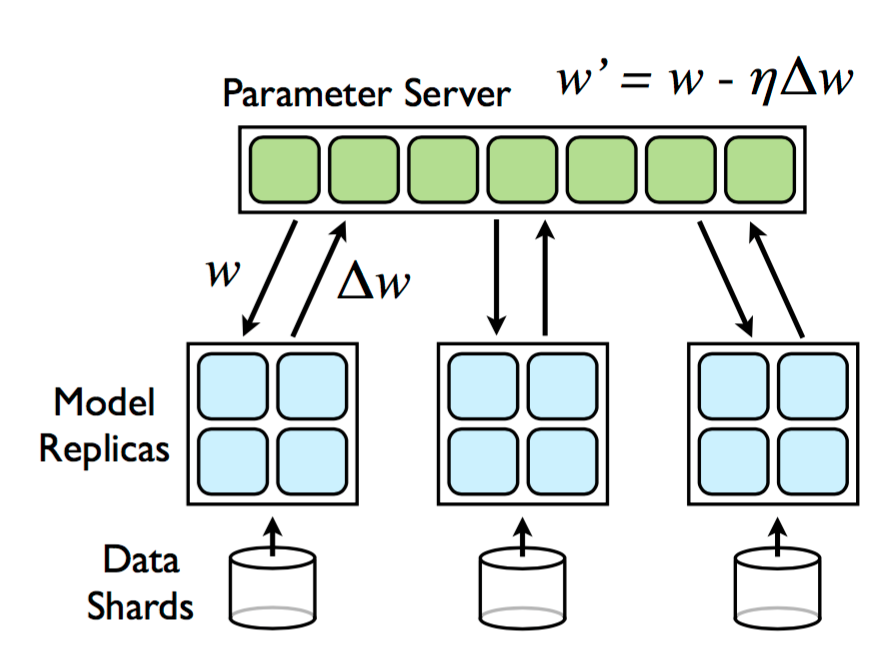
\includegraphics[scale = .6]{./images/downpour}
  \caption{A graphic modeling the functionality of Downpour SGD \cite{distbelief}}
  \label{fig:downpour}
\end{figure}

\noindent This algorithm works by farming out a set of training examples to the children, all of which will start with the same set of parameters. However, as soon as one of the examples returns to the parameter server, it will update global parameters and receive a new example to process with the updated set of parameters. It is important to note that we are no longer locking the parameters when they update, and we are not promised that each of the model replicas are going to have the most up to date set of parameters. However, remembering that this model is relatively sparse, we hope that if the samples are diversified enough, we can distribute out these parameter updates and capture the diversity in the gradients that will move us more quickly towards our target objective. \\

\noindent Shortly after in 2015, Google released their second distributed machine learning model: tensorflow \cite{tensorflow}. This model was much more user friendly, and it had a much heavier focus in distributed systems. In this model, Google uses their most up to date version of Protocol Buffers as the mechanism for passing parameters within the system \cite{protobuf}. For this project, we sought to first combine the DistBelief algorithm, with the distributed systems in tensorflow into our own mock distributed SGD system. We then improved the reliability of our system by implementing Paxos leader selection for server failures, and we then compared the use of the system to other mechanism of sending data, specifically Zeromq \footnote{http://zeromq.org}, a Distributed C-based messaging system. 


\section{Motivation}

For our implementation of Downpour Gradient Descent, we decided to use Python because of the rich support available for both machine learning and distributed system communication. The dataset we decided to work with was the Caltech 101 Computational Vision dataset. This data entailed around 20,000 images of around 101 categories with a size of 300 by 200. The toy example that we applied our implementation of takes approximately 56 minutes to run stochastic gradient descent.

\section{Challenges}

\noindent For this project, we used some of the cheapest Google Cloud servers in order to spawn client machines. We used the 2-core machines with 6.5Gb of RAM. Under these circumstances, building the convolution neural net was particularly straining for the machine. The model parameters are already relatively large themselves, and the intermediate operations in performing gradient descent can be even larger. As a result, instances frequently crashed. In particular, we had to handle the following errors in a graceful way: Network Errors, Memory Errors, Timeouts, Hardware Failure. Consequently, designs to approach stochastic gradient descent needed to be particularly fault tolerant.\\

\noindent Additionally, there were a total of 11 million parameters, or 80Mb of parameters. During each batch, the parameters needed to be passed around from the model server to the parameter server. Passing these parameters is particularly network IO intensive, so we needed to investigate ways to reduce the movement of the parameters. As a result, we had to always assume that the network was unreliable and that the latency was nonzero.\\

\noindent Finally, speed was incredibly important for this system. Gradient descent on one machine took around 56 minutes or 20 seconds per batch on one machine. We needed to optimize our system such that the average speed was higher than this. We also needed to ensure that convergence was achieved at a faster rate. \\

\noindent Ultimately, many of our challenges for this task arose not only from the nontrivial nature of this image classification task, but also the inconsistency of the cloud. As described frequently in class, a lot of the work involved in distributed systems is system administration. This task was far easier on our local machines. The difficulty of this project arose from ensuring that it consistently functioned well across unreliable components.

\section{Methods and Design}

The aforementioned challenges required that the downpour SGD distributed system must be fast. The most critical bottleneck in this implementation was the transfer speed. As mentioned above, we researched with different machine learning implementations and observed how they executed remote procedure calls efficiently. After some research and experimentation, we found gRPC to be the most reliable. gRPC is the framework used by TensorFlow and is heavily used within Google for their systems. \\

\noindent Our initial implementations simply tried to pass 80Mb back and forth using GRPC calls. Simply trying to send the parameters through GRPC took upwards of a minute for our use cases and would frequently fail. Consequently, we attempted to improve speeds by streaming the parameters in chunks. Performing some tuning, we found that a chunk size of 512Kb was the optimal amount to stream the tensors in. This helped reduce the transfer time for over a minute to 1.6 seconds. This made the problem far more reasonable.\\

\begin{figure}[!ht]
  \centering
      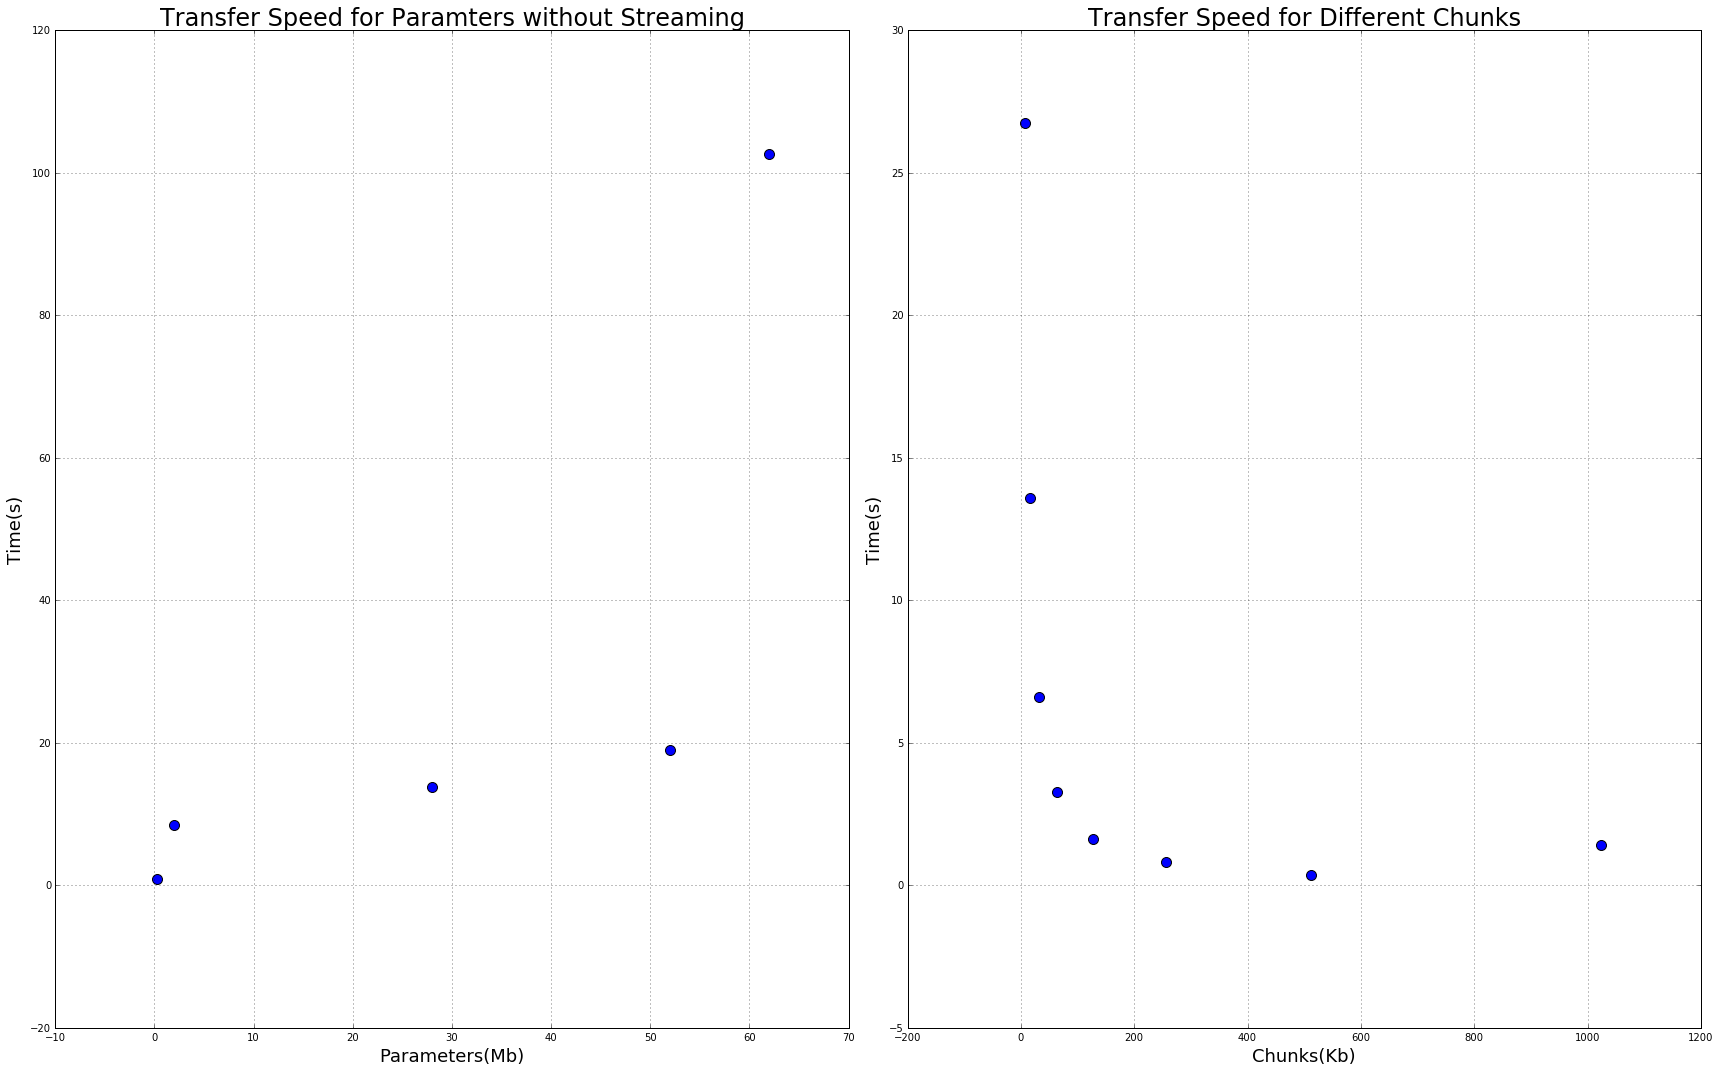
\includegraphics[scale = .2]{./images/speeds.png}
  \caption{On left, transfer speeds for different amounts of parameters. On right, transfer speeds based on chunk size while streaming the parameters.}
  \label{fig:local}
\end{figure}


\noindent gRPC allowed us to organize our model in a logical way. We had multiple clients for each parameter server. Our parameter server took in tensors from the different clients. A parameter server could interact with the clients by sending the clients the most up to date parameters. The client servers sent the parameter server updates from performing gradient descent. \\

\noindent In terms of fault tolerance, we first dealt with the easier scenario: the failure of one of multiple client servers. The effects of a client server failure were much less catastrophic. The impact was simply slower training time and an unresponsive client. We implemented timeouts to ensure that the server would not be blocked by a crashed client server. \\

\noindent Additionally, we implemented simple ways to maximize the uptime of our clients and try to maintain relatively high training speeds. We implemented a bash script that involved an infinite while loop that constantly restarted the client server whenever there was an error. This ensured that if the client failed from a NetworkError or a MemoryError, the client would be quickly restarted as soon as possible.\\

\noindent A more difficult fault to deal with was an arbitrary shutdown of the system. In order to deal with this, we used resources available from Google Cloud Compute. Initially, we began implementing an isolated set of servers that would ping other client servers to see if they were running. If they were not running, these isolated set of set of servers would reinstantiate the computing instance. However, as one might expect, this feature is readily available within Google Cloud Compute. Consequently, we took advantage of this and configured this feature. \\

\noindent Without question, the most challenging fault we needed to deal with in this system was the failure of the parameter server. The failure of the parameter server would be the most catastrophic. Without reinstating or saving the parameter server, all training would be wasted upon the crash of the parameter server. If the failure of the server was not detected, this could halt all training. \\ 

\noindent Our solution to the failure of the parameter server was the Paxos protocol. The Paxos protocol would be launched whenever clients detected in unison that the parameter server was down. Clients would detect the failure of the parameter server by detecting multiple consecutive failed instances to communicate with the parameter server. If multiple consecutive failures happened, the client server would execute the Paxos algorithm to decide a new parameter server. In our case, the proposal number if a float as a simple way to keep all proposal numbers distinct. The proposal value is the proposed server IP address. \\

\noindent The basic steps of the Paxos protocol in context of our program are shown below.
\begin{enumerate}
    \item A majority of client servers have initiated the Paxos protocol because they have not received updates from their parameter server
    \item After confirming that a majority of the clients have initiated, clients make proposal $n$ with value $v$ after a time determined by their seeded value. Client servers that had received updated parameters relatively recently are seeded with a lower random value.
    \item After receiving a proposal, clients acknowledge that they have seen the proposal and send back the largest proposal value $v$ they have seen so far.
    \item If the proposer gets an acknowledgement with a proposal $n'$ larger than it's proposal $n$, the process is stopped. However, if it gets an acknowledgement from the majority of clients and it has provided the largest proposal $n$, then it continues. 
    \item Next the proposer requests acceptance of the proposal from all clients. If the clients have already accepted a prepare value with a higher proposal value, then it rejects. Otherwise, it sends it's largest proposal  $n$ and value $v$.
    \item If the majority of the clients accept the proposal $n$, then that value becomes the new server IP address.
    \item All clients check to see if they are a server. If they are, they begin to serve parameters. Otherwise, clients begin to request parameters from the new server.
    \item If the proposer is rejected, backoff time for the next proposal is increased and the proposal number is increased as well for this client. This process is continued until agreement is achieved.
\end{enumerate}

\noindent The Paxos protocol is also used to initiate training of the model. This keeps things relatively generic and makes the startup script to launch a model across multiple Google Compute instances as simple as calling "python client.py" on each one. Parameter server setup and the coordination of training would be continued from there.

\section{Results and Discussion}


\begin{figure}[!htp]
  \centering
      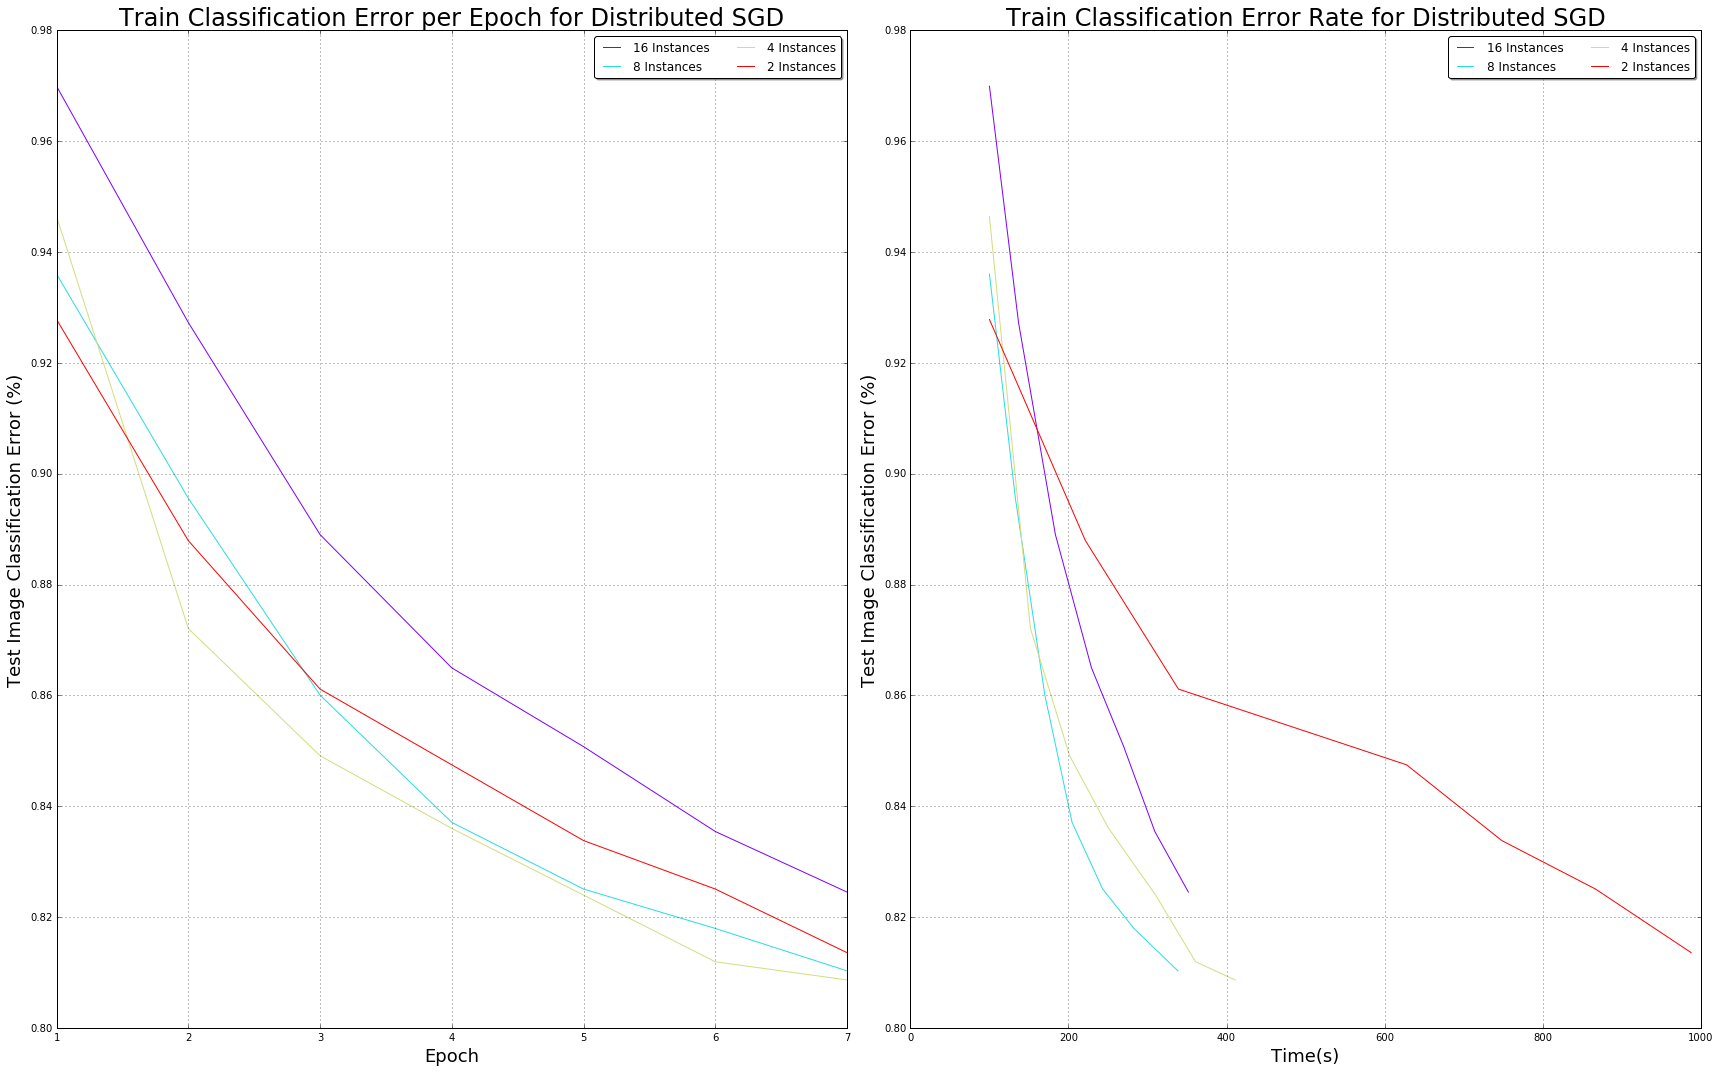
\includegraphics[scale = .2]{./images/sgd_results.png}
  \caption{On left, training classification error rates per epoch. On right, training classification error rates over time.}
  \label{fig:local}
\end{figure}

\noindent From the graph on the right, we can clearly see that generally increasing the number of computing instances can increase the rate at which a model trains. To reach around a image classification error rate of 0.8, the amount of time taken by 8 compute instances was roughly a third of the time required for two instances. One particularly noticeable anomaly is that training the model across 16 compute instances actually trains slower than training across 4 or 8 instances. This seems to suggest that the overhead between the server and clients for communication becomes increasingly nontrivial as the number of compute instances increase. There is a tradeoff between training with more instances. The specific number of instances to use to optimize this tradeoff seems to matter heavily on the amount of time taken to train a batch and the overhead generated from communication and coordination of multiple compute instances.\\

\noindent The graph on the left seems to suggest that as a tradeoff for increased speed, reduction in classification error is not as substantial if there are more servers. This makes sense with our intuition. While running gradient descent on a batch of data, the parameters have not been updated on the previous $n$ batches if there are $n$ compute instances running gradient descent. As shown by the leftmost figure above, we observe the effect of this phenomenon much more substantially when there are 16 compute instance.\\


\noindent Admittedly, though interesting to implement, the Paxos protocol seems to not have the best method for this task. On localhost There was nontrivial overhead to beginning the Paxos procedure across the majority of the clients. Running Paxos itself also frequently took a long time if there were a large number of clients, particularly in the case of 16 clients. Rather, building a robust system that syncs with a parameter server and reinstantiates it if it fails probably would be more efficient. However, the procedure of implementing the Paxos protocol across Google Cloud instances was far more enlightening and a great conclusion to the course. 

\section{Applying SGD in Lua/Torch}

\noindent Next we decided to extend our model to Lua/Torch \footnote{http://torch.ch}, the language we use to build our models for natural language processing. Torch is a much lower-level language, and some of the most computationally heavy operations are done in C. Here, we wanted to experiment with some different system architectures and see if we could find an optimal way to build the Distributed SGD system.\\

\noindent In order to pass parameters between the parameter server and the model clients, we ended up using lua--parallel, a simple parallel computing framework for torch \footnote{https://github.com/clementfarabet/lua---parallel}. This library passes data via ZeroMQ, a fast, asynchronous messaging framework that allows for simple comunication between remote processes. We found this library to be extremely efficient as it took less than 2 seconds to pass a couple million parameters between remote servers using simple socket-like protocols. Beyond this communication protocol, we rewrote all of the same stochastic gradient descent code in Lua.\\ 

\begin{figure}[!htb]
  \centering
      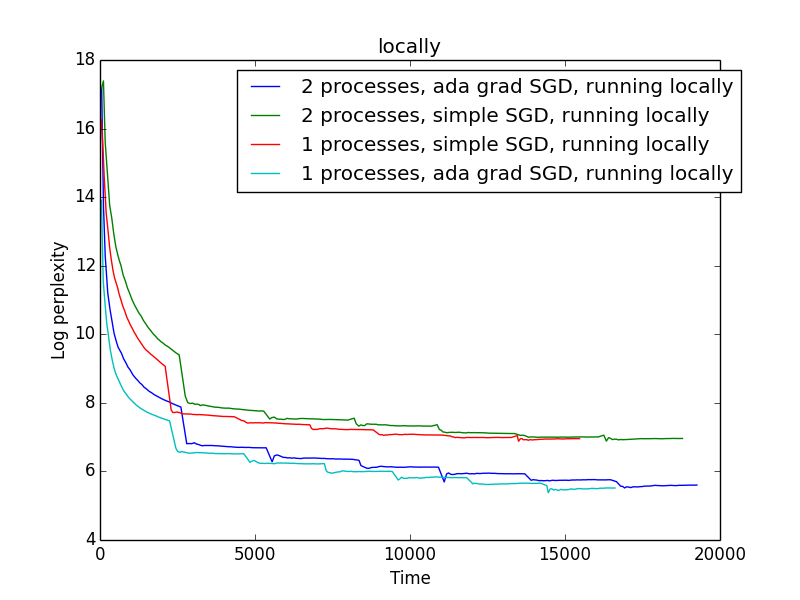
\includegraphics[scale = .5]{./images/locally}
  \caption{The results of running our rnn model for 7 epochs locally.}
  \label{fig:local}
\end{figure}

\noindent For our lua/torch example, we used an encoder-decoder recurrent neural network with the task of machine translation of sentences from English to German. We first set some benchmarks by trying to parallelize out the client systems locally on our own computers. The results of these experiments are displayed in figure ~\ref{fig:local}.\\

\noindent Here, we found the Adagrad SGD algorithm to be particularly useful \cite{adagrad}. In standard SGD, we simply updated our parameters with a fixed learning rate $\eta$, which may decay over time as we become closer and closer to our objective. Adagrad on the other hand tries to eliminate the need for $\eta$ by choosing a dynamic learning rate at the time of the update that is dependent on how much that specific parameter has already tried to be optimized. In comparison the standard SGD algorithm, Adagrad works as follows:\\
\begin{algorithmic}
\State $\mathbf w \gets \mathbf 0$
\State $\mathbf{hist} \gets \mathbf 0$
\While {$\mathbf f(\mathbf w)$ is not minimized}
	\For {$i = 1, n$}
	\State $\mathbf{grad} \gets \nabla f(\mathbf w)$
	\State $\mathbf{hist} \gets \mathbf{hist + grad^2}$
	\State $\mathbf{adj} \gets \mathbf{grad} / \sqrt{\mathbf{hist}}$
    \State $\mathbf w \gets \mathbf w - \eta \mathbf{adj}$
	\EndFor
\EndWhile
\end{algorithmic}

\noindent As seen in figure ~\ref{fig:local}, the adagrad algorithm was a sufficient improvement over the standard SGD algorithm. This is particularly true with the introduction of more and more model replica clients. When there are more clients, there are more out-of-date updates to the parameter server, meaning that a lot of the gradients are going to be repetitive and start to overcompensates for the current error. Adagrad is particularly useful here because it should adjust for an influx of similar gradients. This algorithm will suppress the updates of the errors that are trying to be propogated through the hardest, and then scale the updates that happen relatively infrequently. \\

\noindent In addition, we found that when distributing out this task locally on our machines, there was not much of a speedup in runtime between 1 vs. 2 cores. Even thought the 2 core system had twice as many clients, the clients were competing for resources and it was even slower to run than using a single core. \\

\noindent We then decided to implement our system using remote clients in order to get the full benefits of the distributed system. The results are displayed in figure ~\ref{fig:remote}. From this figure, we can see that by doubling the number of client replicas, we can actually get through 10 epochs in approximately half the time (although not as thoroughly). Even more interestingly, at the initialization, the 8 process system is worse than the 4 process system which is worse than the 2 process system. This intuitively makes sense since by adding more processes, we are overwriting parameter updates making the model train much more slowly. However, as time passes and the historical gradient begins to add up, the systems with more processes start to converge faster and faster as the algorithm learns to ignore the repetitive update arguments. \\

\begin{figure}[!htb]
  \centering
      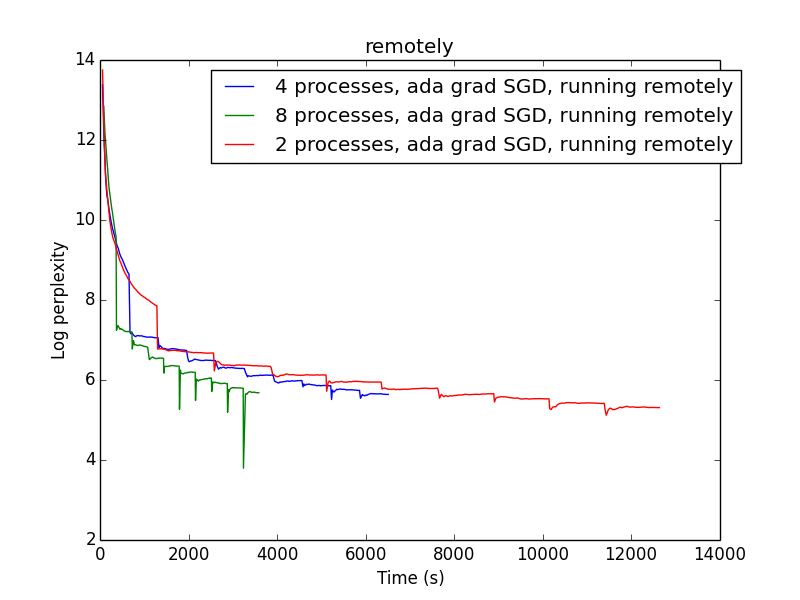
\includegraphics[scale = .5]{./images/remotely}
  \caption{The result of running our rnn model for 10 epochs remotely.}
    \label{fig:remote}
\end{figure}

\noindent The results of this experiment are extremely promising. This shows that by adding additional clients, over the long run, we can continue to increase the speed that the model is training at. More particularly, we hope to extend this model in the future such that it progressively adds more clients as they are needed. Initially, when we have no historical gradients, we do not benefit from having multiple clients as they are all overwriting one another. The standard one-client system works the best at the beginning. With this in mind, it would be optimal to add the new clients in waves as the historical gradient becomes more and more dense. We want there to be less updates when the model has a high learning update rate, and more updates when the model has a low learning update rate.


\section{Conclusion}
As the amount of data continually increases exponentially, machine learning is fundamentally becoming a distributed systems problem. Sometimes, figuring out a complex model that more suitably fits the data can lead to superior results. However, more frequently, a simple model can outperform a more complex model if it can be quickly trained and easily tuned. When the data to train on increases, being able to work on the full dataset  and tune parameters by training multiple models becomes vital. As demonstrated here via both Python and Lua implementations, by distributing the model across multiple compute engines, we can decrease the amount of time it takes to train a model. In order to make models train properly though in a distributed system, we needed to try to implement fault tolerance into our system and apply various distributed systems algorithms. Thourhg this project, we have shown that using techniques learned from class, we can can build a distributed stochastic gradient descent model that works reasonably well.

\section{Code}

All code can be found at the repository linked here: \\ \href{https://github.com/michaelfarrell76/Distributed-SGD}{\color{red} https://github.com/michaelfarrell76/Distributed-SGD}.

\printbibliography

\end{document}
